\documentclass[10pt,a4paper,titlepage]{report}
\usepackage[utf8]{inputenc}
\usepackage{amsmath}
\usepackage{amsfonts}
\usepackage{amssymb}
\usepackage{graphicx}
\usepackage{xcolor}
\usepackage{minted}

\newcommand{\HRule}[1]{\rule{\linewidth}{#1}}

\nonstopmode


\begin{document}
{\fontfamily{cmr}\selectfont
\title{ \normalsize \textsc{}
\\ [2.0cm]
\HRule{0.5pt} \\
\LARGE \textbf{\uppercase{constraints and views}
\HRule{2pt} \\ [0.5cm]
\normalsize \today \vspace*{5\baselineskip}}
}

\date{}

\author{
	Rwithik Manoj \\
	College of Engineering, Trivandrum \\
	Department of Computer Science and Engineering }

\maketitle
\newpage

\sectionfont{\scshape}

\begin{enumerate}
\item
\begin{enumerate}
	\item Create a table named Subjects with the given attributes
		\begin{itemize}
			\item Subid( Should not be NULL)
			\item Subname (Should not be NULL)
		\end{itemize}
		Populate the database. Make sure that all constraints are working properly.\newline
	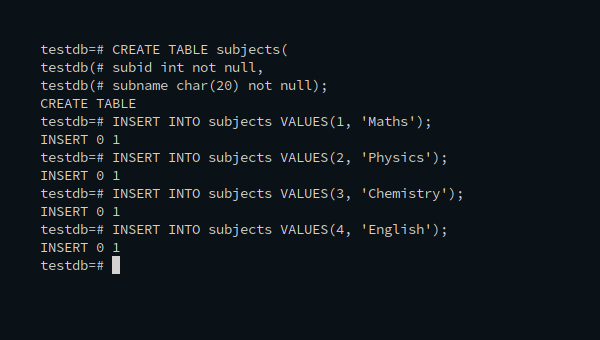
\includegraphics[width=\linewidth]{../Images/Constraints/1.png}\newline
		\begin{enumerate}
			\item Alter the table to set subid as the primary key.\newline
			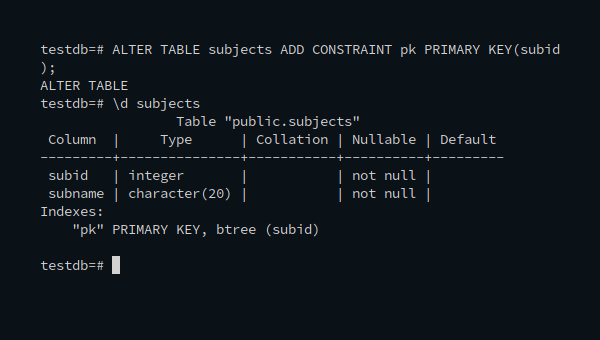
\includegraphics[width=\linewidth]{../Images/Constraints/2.png}\newline
		\end{enumerate}
	\item Create a table named Staff with the given attributes:
		\begin{itemize}
			\item staffid (Should be UNIQUE)
			\item staffname
			\item dept
			\item age (Greater than 22)
			\item salary (Less than 35000)
		\end{itemize}
		Populate the database. Make sure that all constraints are working properly.\newline
		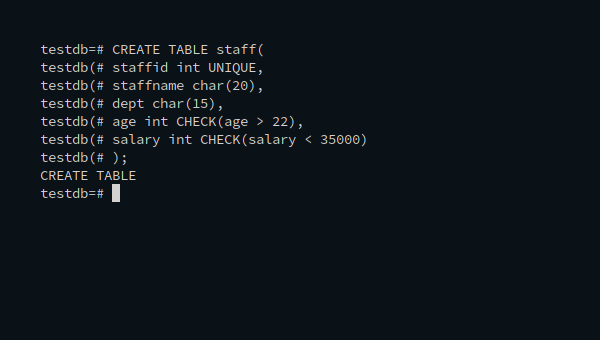
\includegraphics[width=\linewidth]{../Images/Constraints/3.png}\newline
		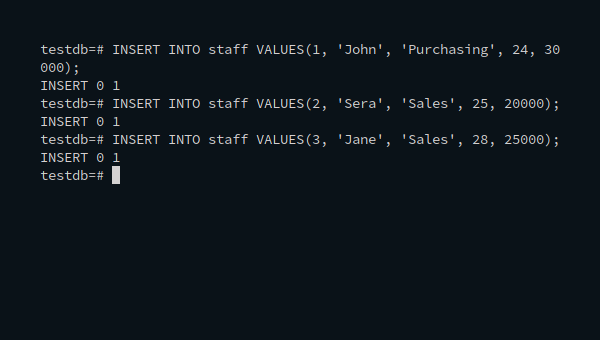
\includegraphics[width=\linewidth]{../Images/Constraints/4.png}\newline
		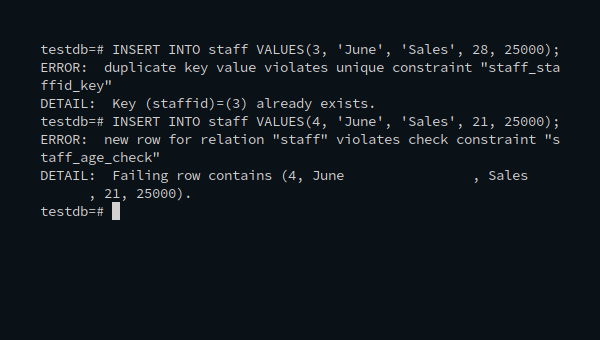
\includegraphics[width=\linewidth]{../Images/Constraints/5.png}\newline
		\begin{enumerate}
			\item Delete the check constraint imposed on the attribute salary\newline
			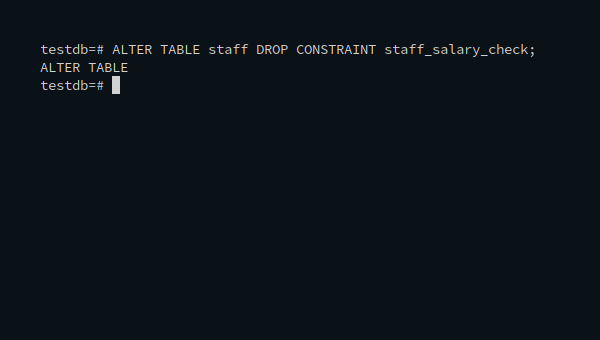
\includegraphics[width=\linewidth]{../Images/Constraints/6.png}\newline
			\item Delete the unique constraint on the attribute staffid\newline
			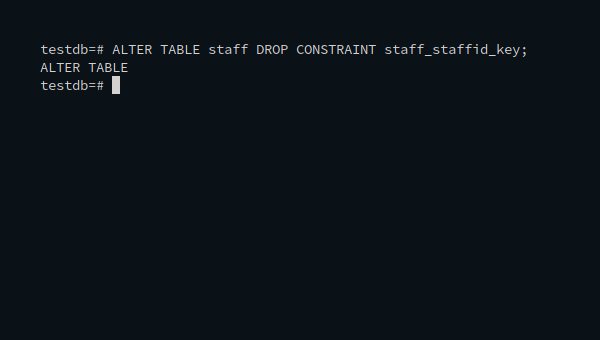
\includegraphics[width=\linewidth]{../Images/Constraints/7.png}\newline
		\end{enumerate}
	\item Create a table named Bank with the following attributes
		\begin{itemize}
			\item bankcode (To be set as Primary Key, type= varchar(3) )
			\item bankname (Should not be NULL)
			\item headoffice
			\item branches (Integer value greater than Zero)
		\end{itemize}
			Populate the database. Make sure that all constraints are working properly.All constraints have to be set after creating the table.\newline
			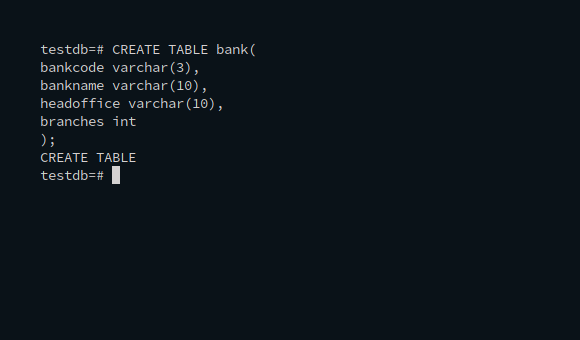
\includegraphics[width=\linewidth]{../Images/Constraints/8.png}\newline
			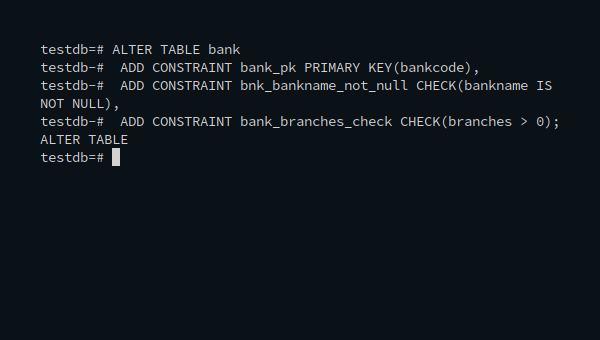
\includegraphics[width=\linewidth]{../Images/Constraints/9.png}\newline
			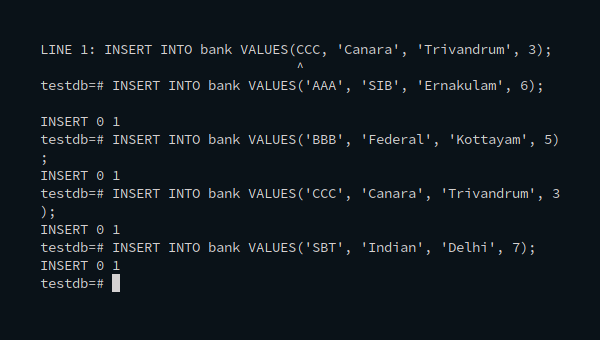
\includegraphics[width=\linewidth]{../Images/Constraints/10.png}\newline
	\item Create a table named Branch with the following attributes
		\begin{itemize}
			\item branchid (To be set as Primary Key)
			\item branchname (Set Default value as ‘New Delhi’)
			\item bankid (Foreign Key:- Refers to bank code of Bank table)
		\end{itemize}
		\begin{enumerate}
			\item Populate the database. Make sure that all constraints are working properly.\newline
			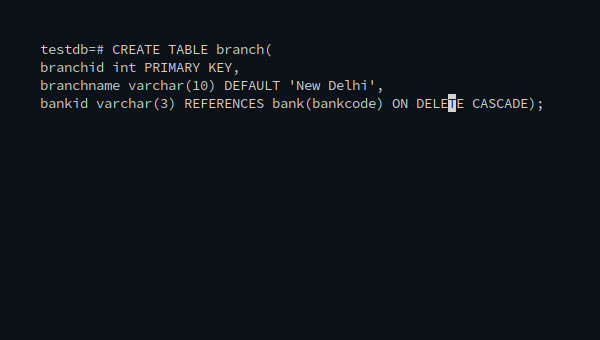
\includegraphics[width=\linewidth]{../Images/Constraints/11.png}\newline
			\item During database population, demonstrate how the DEFAULT Constraint is satisfied.\newline
			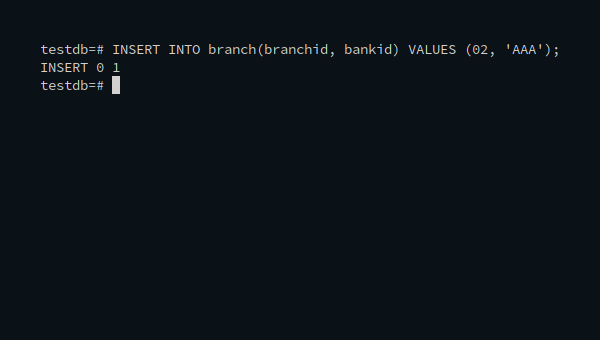
\includegraphics[width=\linewidth]{../Images/Constraints/12.png}\newline
			\item Delete the bank with bank code ‘SBT’ and make sure that the corresponding entries are getting deleted from the related tables.\newline
			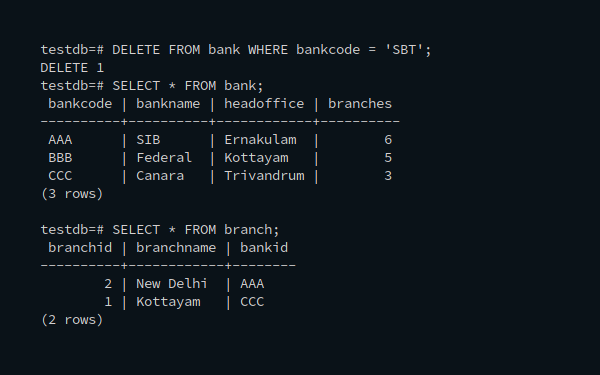
\includegraphics[width=\linewidth]{../Images/Constraints/13.png}\newline
			\item Drop the Primary Key using ALTER command\newline
			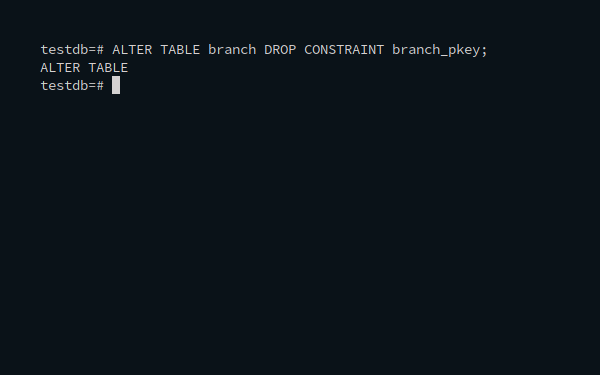
\includegraphics[width=\linewidth]{../Images/Constraints/14.png}\newline
		\end{enumerate}
\end{enumerate}
\item Create a View named sales\_staff to hold the details of all staff working in sales Department\newline
	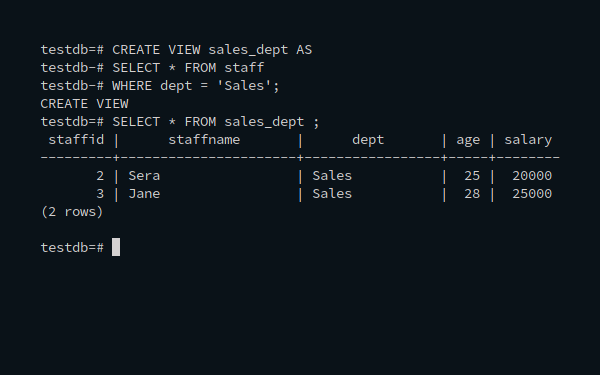
\includegraphics[width=\linewidth]{../Images/Constraints/15.png}\newline

\item Drop table branch. Create another table named branch and name all the constraints as given below:
	\begin{itemize}
		\item Constraint name Column Constraint
		\item Pk branch\_id Primary key
		\item Df branch\_name Default :’New Delhi’
		\item Fk bankid Foreign key/References
	\end{itemize}
	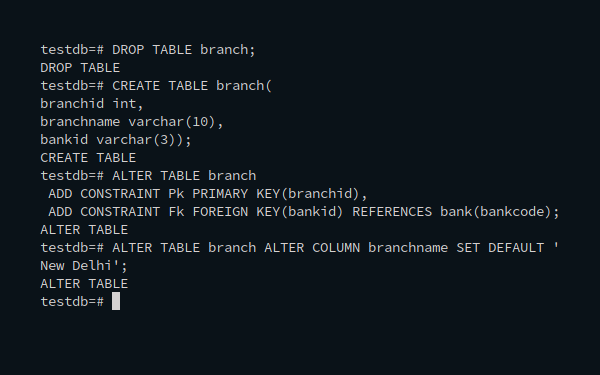
\includegraphics[width=\linewidth]{../Images/Constraints/16.png}\newline
	\begin{enumerate}
		\item Delete the default constraint in the table\newline
		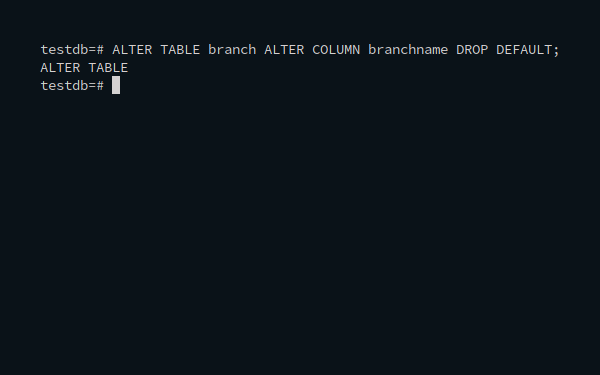
\includegraphics[width=\linewidth]{../Images/Constraints/17.png}\newline
		\item Delete the primary key constraint\newline
		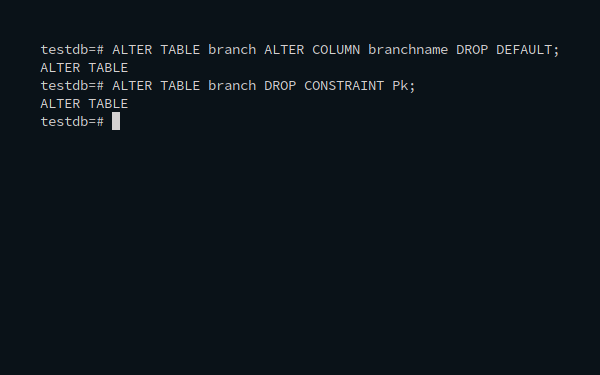
\includegraphics[width=\linewidth]{../Images/Constraints/18.png}\newline
	\end{enumerate}

\item Update the view sales\_staff to include the details of staff belonging to sales department whose salary is greater than 20000.\newline
	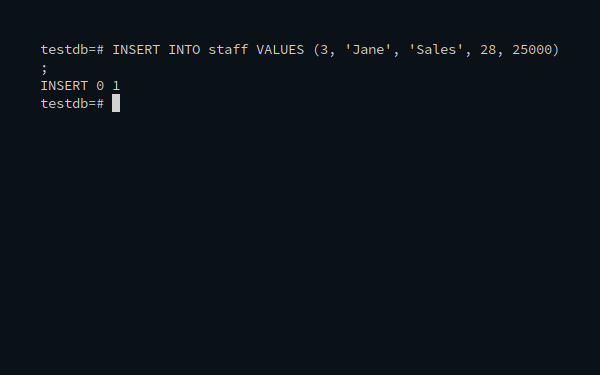
\includegraphics[width=\linewidth]{../Images/Constraints/19.png}\newline
\item Delete the view sales\_staff.\newline
	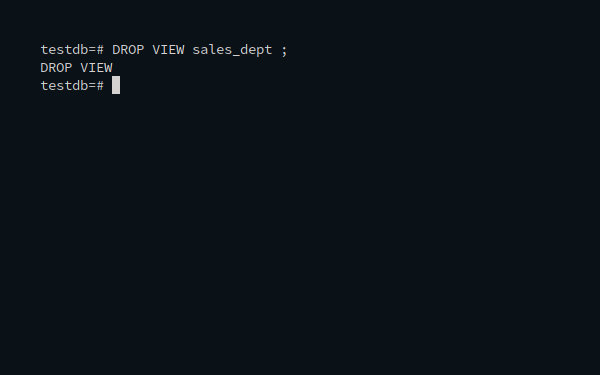
\includegraphics[width=\linewidth]{../Images/Constraints/20.png}\newline

\end{enumerate}



}
\end{document}
